\documentclass[notitlepage,a4paper,11pt,hyperref=pdftex]{revtex4-1}
\usepackage{docs}
\usepackage[T2A]{fontenc}
\usepackage[utf8x]{inputenc}
% Русский язык
% \usepackage[english,russian]{babel}

% Математические сиволы 
\usepackage{amssymb,amsfonts,amsmath,mathtext}
\usepackage{textcomp}
% Гиперссылки
\usepackage[unicode, bookmarks=true,colorlinks,linkcolor=red,citecolor=green,urlcolor=blue]{hyperref}
\usepackage{bbold}

% Изображения
\usepackage[pdftex]{graphicx}

% Цвета
\usepackage[usenames]{color}
\usepackage{colortbl}


% Для квантовой физики
\renewcommand{\tan}{\mathop{\rm tg}\nolimits}
\newcommand{\bra}[1]{\langle#1|}
\newcommand{\ket}[1]{|#1\rangle}
\newcommand{\bracket}[2]{\langle#1|#2\rangle}
\newcommand{\mean}[1]{\langle#1\rangle}
\newcommand{\means}[1]{\langle#1\rangle_{sym}}
\newcommand{\Tr}[1]{\textbf{Tr}\{#1\}}
\newcommand{\dt}[1]{\frac{\partial #1}{\partial t}}
\newcommand{\I}[2]{\int\limits_{#1}^{#2}\,}

\usepackage{hhline}
\usepackage{lineno} % adding line number


% \linenumbers

% \ligodccnumber{T}{12}{000000}{}{v1}
% \ligodistribution{AIC, ISC}
\graphicspath{{images/}}
% \bibliographystyle{phaip}





% \author{Mikhail Korobko}

\begin{document}
\title{Adaptive quantum measurements: progress and questions.}
\maketitle
\section{General procedure}
In this section I just remind what do we have by now.

Our system output  after homodyne detector is: 
\begin{multline}\label{init_y}
 y(t)=\hat{a}_1(t)\cos \zeta(t)+\Bigl[\hat{a}_2(t)+\frac{\alpha}{\hbar}\bigl(\hat{x}(0) \cos \omega_m t+ \frac{\hat{p}(0)}{m \omega_m} \sin \omega_m t + \alpha \int\limits_0^{\infty} dt' \, G(t-t') \Theta(t-t')\, \hat{a}(t') +\\+ \frac{\bar{F}}{m\omega_m}\sin\omega_m(t-\tau)\Theta(t-\tau)\bigr)\Bigr]\sin\zeta(t),
\end{multline}

The estimation procedure is following:
\begin{enumerate}
 \item We estimate arrival time $\tau$ from output
 \item Using this arrival time to find the optimal homodyne angle
\end{enumerate}

\subsection{Stage 1}
We can rewrite signal in general form:
\begin{equation}
 y(t)=\mathbb{C}(t)x+n(t)
\end{equation}
Here:
\begin{align}
& \mathbb{C}(t) = \sin\zeta(t)
\begin{bmatrix}
 \sin\omega_mt, & -\cos\omega_mt
\end{bmatrix}
\\
&
x=
\begin{bmatrix}
 A_c\\
A_s
\end{bmatrix}
\\
& n(t) = 
\begin{bmatrix}
 \cos\zeta(t), & \sin\zeta(t)
\end{bmatrix}
\begin{bmatrix}
 n_1(t)\\
n_2(t)
\end{bmatrix}
% =\mathbb{F}(t)\mathbb{N}(t)
\end{align}
and 
\begin{align}
 & A_c = \frac{\bar{F}}{m\omega_m}\cos\omega_m\tau\,\Theta(t-t'),\\
& A_s = \frac{\bar{F}}{m\omega_m}\sin\omega_m\tau\,\Theta(t-t'),
\end{align}

We use BLUE (best linear unbiased estimation) for estimating the parameters of this signal:
\begin{equation}
 \tilde{x} =
\begin{bmatrix}
 \tilde{A_c}\\
\tilde{A_s}
\end{bmatrix}
= (\mathbb{D}^T\mathbb{N}^{-1}\mathbb{D})^{-1}\mathbb{D}^T\mathbb{N}^{-1}\mathbf{y}
\end{equation}

Here
\begin{equation}
 \mathbb{D} = 
\begin{bmatrix}
 \mathbb{C}(t_0) \\
 \mathbb{C}(t_1) \\
 \vdots\\
 \mathbb{C}(t)
\end{bmatrix},
\qquad
 \mathbf{y} = 
\begin{bmatrix}1
 y(t_0)\\
 y(t_1)\\
\vdots\\
y(t)
\end{bmatrix},
\qquad
 \mathbb{N} = 
\begin{bmatrix}
 \mean{n(t_0),n(t_0)} & \mean{n(t_0),n(t_1)} & \hdots & \mean{n(t_0),n(t)} \\
\mean{n(t_1),n(t_0)} & \mean{n(t_1),n(t_1)} & \hdots & \mean{n(t_1),n(t)} \\
\vdots & \vdots & \ddots & \vdots \\
\mean{n(t),n(t)} & \mean{n(t_1),n(t)} & \hdots & \mean{n(t),n(t)} \\
\end{bmatrix}
\end{equation}
where
\begin{equation}
 \mean{n(t_i)n(t_j)} = 
\begin{bmatrix}
 \cos\zeta(t), & \sin\zeta(t)
\end{bmatrix}
\begin{bmatrix}
 \mean{n_1(t_i),n_1(t_j)} & \mean{n_1(t_i),n_2(t_j)}\\
 \mean{n_2(t_i),n_1(t_j)} & \mean{n_2(t_i),n_2(t_j)}
\end{bmatrix}
\begin{bmatrix}
 \cos\zeta(t_j)\\ \sin\zeta(t_j)
\end{bmatrix}
\end{equation}

and

\begin{equation}\label{noises}
 \begin{cases}
  \means{\hat{n}_1(t)\hat{n}_1(t')}=&\frac{1}{2}\delta(t-t'),\\
  \means{\hat{n}_1(t)\hat{n}_2(t')}=&\frac{\alpha^2}{2\hbar}G(t'-t)\Theta(t'-t),\\
  \means{\hat{n}_2(t)\hat{n}_1(t')}=&\frac{\alpha^2}{2\hbar}G(t-t')\Theta(t-t'),\\
  \means{\hat{n}_2(t)\hat{n}_2(t')}=&\frac{1}{2}\delta(t-t')+\frac{\alpha^4}{4\hbar^2 m^2 \omega_m^2}\bigl(t'\cos\omega_m(t-t')-\frac{1}{\omega_m}\cos\omega_mt\sin\omega_mt'\bigr)\Theta(t-t')+\\
&+\frac{\alpha^4}{4\hbar^2 m^2 \omega_m^2}\bigl(t\cos\omega_m(t-t')-\frac{1}{\omega_m}\cos\omega_mt'\sin\omega_mt\bigr)\Theta(t'-t)+\\&+ \frac{\alpha^2}{2 m w \hbar}\cos\omega_m(t-t').
 \end{cases}
\end{equation}

Then we know the two values $A_{c,x}$ and can get the estimation for arrival time.
\begin{equation}
 \tilde{\tau} = \frac{1}{\omega_m}\arctan \frac{\tilde{A}_s}{\tilde{A}_c}
\end{equation}

\subsection{Stage 2}
On this stage we want to find the optimal homodyne angle for the next moment of time. We suggest two possibilities (both have pro and contra arguments):
\begin{enumerate}
 \item Use variational approach to achieve the back action evasion. We can calculate simple formula for dependence of homodyne angle on time:
\begin{equation}\label{g2}
 g_2(t) = \frac{4\omega_m\hbar}{\alpha} \frac{\sin\omega_m(t-\tau)}{2\omega_mT-\sin2\omega_m(T-\tau)-\sin2\omega_m\tau}
\end{equation}
\begin{equation}\label{g1}
 g_1(t) = \frac{\alpha}{m \omega_m} \frac{-2\omega_m(t-T)\cos\omega_m(t-\tau) + \sin\omega_m(t-\tau) + \sin\omega_m(t-2T+\tau)}{-2T\omega_m + \sin2\omega_m(T-\tau)+\sin2\omega_m\tau}
\end{equation}
So,we can get analytical equation for homodyne angle from Eq.\ref{g1},\ref{g2}:
\begin{equation}\label{appx:zeta}
 \zeta(t) = \arctan\frac{g_2(t)}{g_1(t)}
\end{equation}

At each time step we calculate the arrival time and then calculate the homodyne angle for the next moment of time $t+dt$
\item Knowing the arrival time, we can calculate the $b_{1,2}$ quadratures for any moment of time in future. We suppose, that we can measure both these two quadratures at the same time, so if we construct
the signal consisting of measured values in past and predicted quadratures in future, we can get optimal filtering function. This optimal function will give us best possible estimation in future.
\begin{multline}\label{x0filt}
 \tilde{x}_0 = (\mathbb{D}^T\mathbb{N}^{-1}\mathbb{D})^{-1}\mathbb{D}^T\mathbb{N}^{-1}\mathbf{y} = \\ =
\begin{bmatrix}
 L_1, & L_2, & \hdots & L_N, & L_{N+1}, & L_{N+1}^{'}, & L_{N+2}, & L_{N+2}^{'}
\end{bmatrix}
\begin{bmatrix}
 y(t_1)\\\vdots\\ y(t) \\ \hat{b}_1(t+dt)\\ \hat{b}_2(t+dt)\\ \hat{b}_1(t+2dt)\\ \hat{b}_2(t+2dt)
\end{bmatrix}
=\\ =Y_N + L_{N+1}\hat{b}_1(t+dt)+L_{N+1}^{'}\hat{b}_2(t+dt)+L_{N+2}\hat{b}_1(t+2dt)+L_{N+2}^{'}\hat{b}_2(t+2dt)
\end{multline}

From the other hand, in reality we, of course, can't measure both $b_{1,2}$ quadratures. So, in reality our estimation procedure would be:
\begin{multline}\label{x0meas}
 \tilde{x}_0 = \mathbb{K}\mathbf{y}_r = \mathbb{K}_N\mathbf{y}_N + K_{N+1}\hat{b}_1(t+dt)\cos\zeta(t+dt)+K_{N+1}\hat{b}_2(t+dt)\sin\zeta(t+dt)+\\+ K_{N+2}\hat{b}_1(t+2dt)\cos\zeta(t+dt)+K_{N+2}\hat{b}_2(t+dt)\sin\zeta(t+2dt)
\end{multline}
We are interested in only the part of this equation with time $t+dt$. Obviously, from last two equation we get:
\begin{equation}
 \tan \zeta(t+dt) = \frac{L_{N+1}}{L_{N+1}^{'}}
\end{equation}
\end{enumerate}
\section{Some results}
\begin{figure}
 \begin{minipage}{0.45\linewidth}
  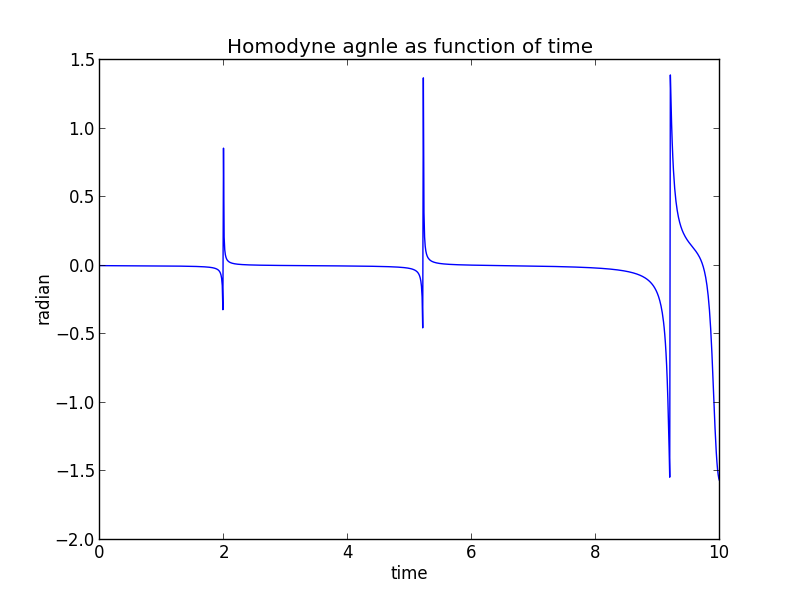
\includegraphics[width=1.\linewidth]{homodyne_angle_var}
 \end{minipage}
\hfill
 \begin{minipage}{0.45\linewidth}
  \center{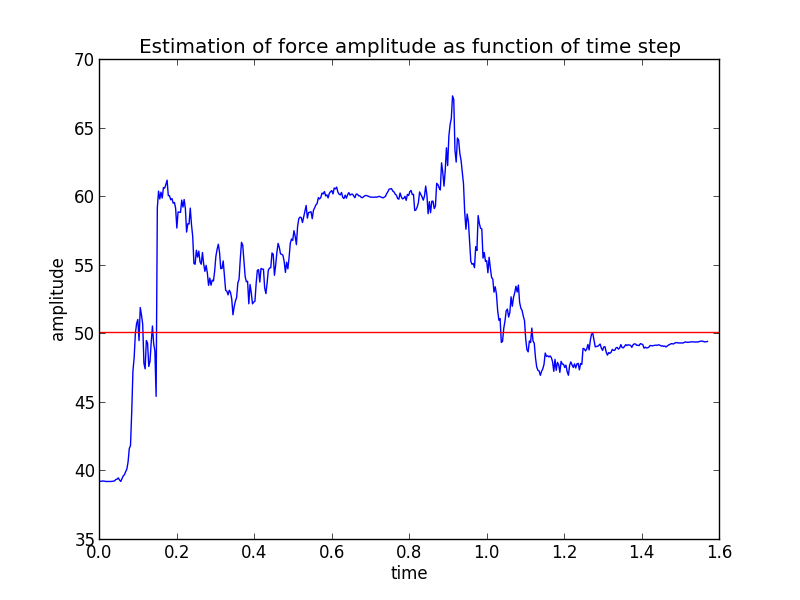
\includegraphics[width=1.\linewidth]{force_estimation}}
 \end{minipage}
\caption{Homodyne angle $\zeta(t)$ dependence of time \textit{(left)} and estimation of delay time depending on time \textit{(right)} (one period).}
\label{pic:hom}
\end{figure}
\begin{figure}
 \begin{minipage}{0.45\linewidth}
  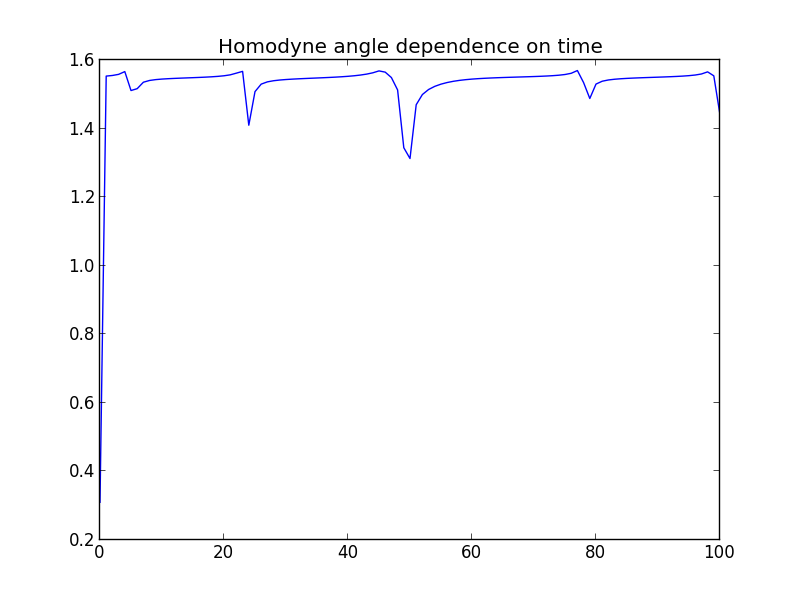
\includegraphics[width=1.\linewidth]{z_a1}
 \end{minipage}
\hfill
 \begin{minipage}{0.45\linewidth}
  \center{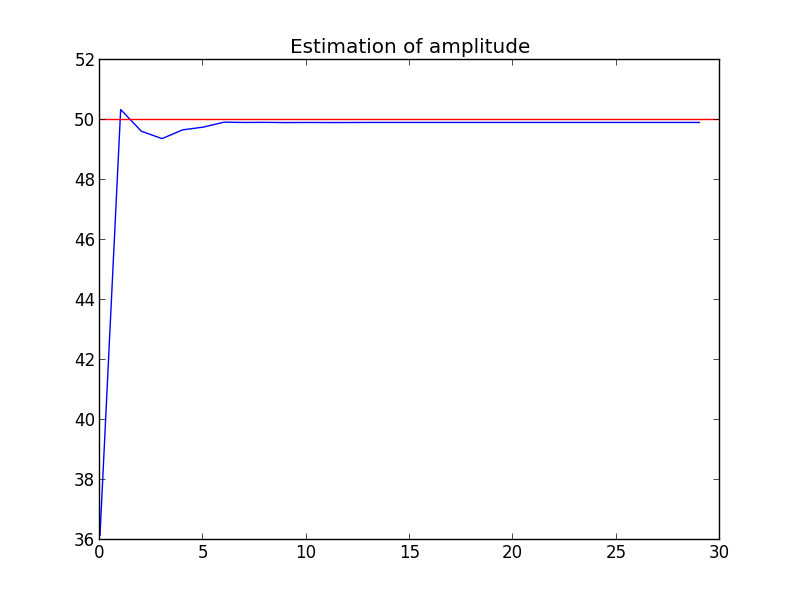
\includegraphics[width=1.\linewidth]{F_a10_big}}
 \end{minipage}
\caption{Homodyne angle $\zeta(t)$ dependence of time \textit{(left)} and estimation of delay time depending on time \textit{(right)} (one period).}
\label{pic:filt}
\end{figure}
I wrote the program that proceeds all pointed above.

If we use the variational readout on the second stage Fig.\ref{pic:hom} and if we use filtering Fig.\ref{pic:filt}
But there's the problem: fine, we've just got some new figure (or statistics), but how do we know if it's correct? Is there any mistake in program? Or may be method gives wrong result...

\section{Questions and problems}
I think that the main problem here now is impossibility to check if our code works fine: we have nothing to compare with. That's why I leave the questions of statistics, arrival time, and the other important things
for future consideration. Now there're few questions we have to concentrate on to achieve some result.

\begin{itemize}
 \item How can we check if our result is correct or not? I think we have no other possibility than to calculate some analytical formula, because any numerical result will rise the same question: 
are we sure, that our code has no mistakes or bugs?

\begin{enumerate}
 \item we can calculate the analytical form of the filtering function (see Appendix \ref{appx:filters})
 \item or we can consider some general and simple case of adaptive measurements - for the simple mechanical system. We proceed two measurements: first weak one, obtaining some information about two quadratures (say 
$x, p$). Because this measurement is quite weak, we disturb the state not that much. Then we can use the information about the quadratures to proceed the second measurement, strong one, that will give us possibly better
precision.
\end{enumerate}
In the first case we get analytical structure for the answer, but have to deal with initial conditions somehow. The second one gives us possibility to investigate the features of adaptive measurements in general,
but gives us only order of magnitude estimation for quality of our particular task.

\item Which procedure on the second stage we should use?

From one point of view, variational method provides us analytical formula that we can use quite simply in our procedure, but how do we know if it is optimal in our case?
From the other point of view, using filter is even less clear: how can we be sure, that in Eq. \ref{x0filt} and \ref{x0meas} $Y_N=\mathbb{K}_N\mathbf{y}_N$? 

\item How to deal with initial conditions?

If we say that our filter is optimal, it should eliminate the initial conditions. But that means this filter should be some kind of differential operator. But from analytical solution 
we can't get the differential operator.
\end{itemize}
\newpage
\appendix
\section{Caclulating the analytical filter}\label{appx:filters}
\begin{figure}
 \center{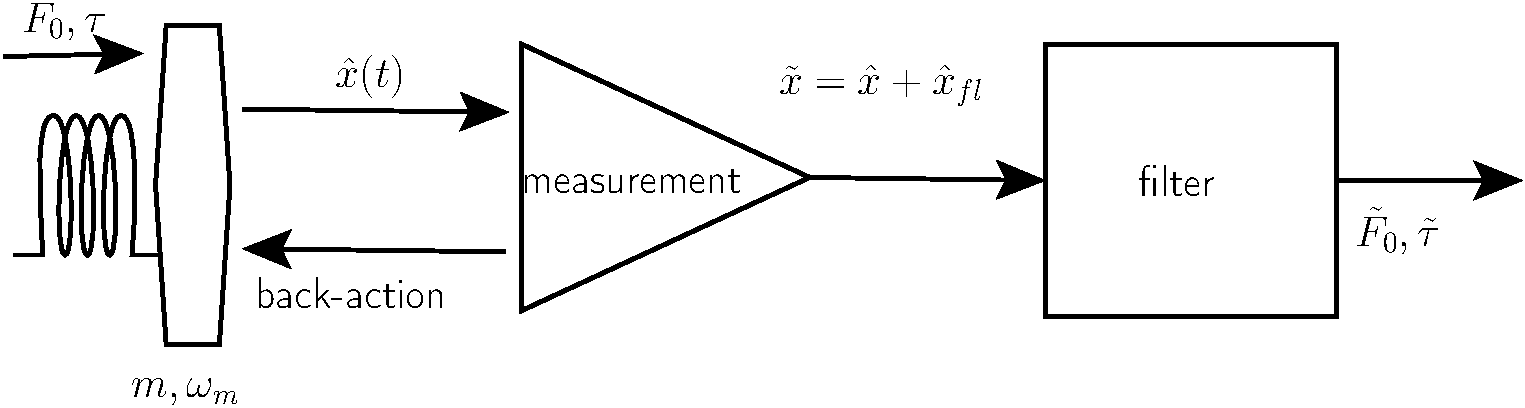
\includegraphics[width=0.8\textwidth]{measurement}}
\caption{General system}
\label{fig:meas}
\end{figure}

Let's consider simple case, without any particular measuring device (see Fig.\ref{fig:meas}). All we know about it is than it measures position of the oscillator and it has spectral densities of noises: $S_x,S_F, S_{xF}$
then we can calculate the optimal unbiased estimate minimizing the variation.

Our system is described by the following equation:
\begin{equation}
 \mathbf{D}\hat{x}(t) = m\ddot{\hat{x}}(t) + m \omega_m^2 \hat{x}(t) = F_s(t) + \hat{F}_{fl}(t), 
\end{equation}
where $F_s(t) = F_0\delta(t-\tau)$ is our signal force and we want to estimate it's amplitude $F_0$

We can write down the general solution for this equation:
\begin{equation}
 \hat{x}(t) = \hat{x}(0)\cos\omega_mt + \frac{\hat{p}(0)}{m\omega_m}\sin\omega_mt + \mathbf{D}^{-1}(F_s(t) + \hat{F}_{fl}(t))
\end{equation}
Here we notice, that $\hat{x}(t)$ is coordinate of the oscillator, and after measuring device it is $\tilde{x}(t) = \hat{x}(t)+\hat{x}_{fl}(t)$
Then we have to get rid of initial conditions. Normally it can be done by applying operator $\mathbf{D}$ to the output signal $\tilde{x}(t)$. But in this case we get 
\begin{equation}
 \tilde{F}(t) = \mathbf{D}\tilde{x}(t) = F_s(t) + \hat{F}_{fl}(t) + \mathbf{D}\hat{x}_{fl}(t)
\end{equation}
and we get the delta function with unknown parameter, that can't be simply linearized. 
Even if we apply the spectral approach here, we get:
\begin{equation}
 F_s(\omega) = \I{-\infty}{\infty}dt\,F_0\delta(t-\tau)e^{-\imath\omega t} = F_0 e^{-\imath\omega \tau} = F_0 (\cos\omega\tau - i \sin\omega\tau) = A_c(\omega) - i A_s(\omega)
\end{equation}
But how to deal with these quadratures, how to get filters - is not clear for me.

That's why we now can say just ``let's consider it insufficient'' and throw these terms:
\begin{multline}
 \tilde{x}(t) = \hat{x}_{fl}(t) + \frac{1}{m\omega_m}\I{0}{t}dt'\,(F_s(t') + \hat{F}_{fl}(t'))\sin\omega_m(t-t') =\\
= \hat{x}_{fl}(t) + \frac{1}{m\omega_m}(F_0\cos\omega_m\tau \sin\omega_mt - F_0\sin\omega_m\tau\cos\omega_mt) + \frac{1}{m\omega_m}\I{0}{t}dt'\,\hat{F}_{fl}(t')\sin\omega_m(t-t')
\end{multline}
or we can change $A_c = \frac{1}{m\omega_m}F_0\cos\omega_m\tau$ and $A_s = \frac{1}{m\omega_m}F_0\sin\omega_m\tau$ and get linear equation:
\begin{equation}
 \tilde{x}(t)=\hat{x}_{fl}(t) + A_c\sin\omega_mt - A_s\cos\omega_mt + \frac{1}{m\omega_m}\I{0}{t}dt'\,\hat{F}_{fl}(t')\sin\omega_m(t-t')
\end{equation}
then we proceed filtering:
\begin{equation}
 \begin{cases}
  \tilde{A}_c = \I{-\infty}{\infty}\,g_1(t')\tilde{x}(t')\,dt'\\
\tilde{A}_s = \I{-\infty}{\infty}\,g_2(t')\tilde{x}(t')\,dt'
 \end{cases}
\end{equation}
in order to get unbiased estimation, which means that $\tilde{A}_{c,s} = \bar{A}_{c,s} = A_{c,s}$, we should have constraints for the filtering functions:
\begin{align}
 \I{-\infty}{\infty}g_1(t')\sin\omega_mt'\,dt' =& 1\\
 \I{-\infty}{\infty}g_2(t')\cos\omega_mt'\,dt' =&1
\end{align}
Then for variations (we omit the formulas for $A_s$,because they are similar to that with $A_c$):
\begin{multline}
 \mean{(A_c-\tilde{A}_c)^2} = \I{-\infty}{\infty}dt\,g_1(t)\,\bigl(\mean{\hat{x}_{fl}^2} +\frac{1}{m^2\omega_m^2}\iint\limits_{0}^{t}dt'\,dt''\,\mean{F_{fl}(t'),F_{fl}(t'')}\sin\omega_m(t-t')\sin\omega_m(t-t'')+\\
+ \frac{2}{m\omega_m}\I{0}{t}dt'\,\mean{F_{fl}(t'),x_{fl}(t)}\sin\omega_m(t-t')\bigr) 
\end{multline}
We assume, that knowing spectral densities we can calculate correlation functions and all the big term inside parentheses in previous equation (let's call it $K(t)$):
\begin{equation}
 \mean{(A_c-\tilde{A}_c)^2} = \I{-\infty}{\infty}dt\,g_1(t)\,K(t)
\end{equation}
then we construct the Lagrange function:
\begin{equation}
 L[g_1(t)] = \I{-\infty}{\infty}dt\,g_1(t)\,K(t) + \lambda(\I{-\infty}{\infty}g_1(t')\sin\omega_mt'\,dt' -1)
\end{equation}
and variate it over $g_1$:
\begin{equation}
 \delta L[g_1(t)] = \I{-\infty}{\infty}dt(2g_1(t)\,K(t) + \lambda\sin\omega_mt)\delta g_1(t) = 0
\end{equation}
Then, using the main lemma of calculus of variations, we get:
\begin{equation}
\begin{cases}
 2 g_1(t)K(t) + \lambda\sin\omega_mt = 0\\
\I{-\infty}{\infty}g_1(t')\sin\omega_mt'\,dt' =1
\end{cases}
\end{equation}
 if we know the the $K(t)$ this system can be simply solved and we get the filtering function.
\end{document}